\section{Background}

\subsection{Financial Markets and Trading}

Financial markets play a pivotal role in the modern economy, acting as the backbone for capital flow, liquidity, and risk management. These markets serve as platforms where entities like individuals, companies, and governments can interact to conduct asset exchanges, hedge against financial risks, and fund their operations or projects.

The financial landscape boasts a vast array of markets each serving unique economic functions: \textbf{Stock Markets}, platforms for trading company shares, are essential for capital raising; \textbf{Bond Markets}, where entities borrow from investors via debt instruments; \textbf{Commodities Markets}, for trading essential raw materials and agricultural goods; \textbf{Forex Markets}, the vast networks enabling currency exchange for international trade; \textbf{Derivatives Markets}, where contracts tied to underlying asset values are traded for hedging or speculation; \textbf{Indices Markets}, which aggregate and track market or sector performance; and \textbf{Cryptocurrency Markets}, digital platforms for exchanging cryptocurrencies, indicative of the evolving nature of financial assets powered by blockchain technology.

Each market serves a specific economic function, contributing to efficient capital allocation and reflecting the global economy's health. However, they are deeply interconnected; a fluctuation in one market can ripple through others, as seen in the global reach of the 2008 financial crisis and the volatile movements in cryptocurrency markets. Such events underscore the systemic importance of these markets and their impact on the global economy.

Market participants, ranging from retail investors to large financial institutions like banks and hedge funds, shape the markets' dynamics through their investment decisions and strategies. Their collective actions can influence asset prices, market trends, and the overall direction of the financial markets.

Regulation and oversight are essential to these markets' health and stability. Regulatory bodies across the globe work to ensure fair practices, transparency, and stability within the markets. They implement policies and regulations to protect investors, maintain order, and foster a trustworthy environment conducive to economic growth.

Technological advancements have brought significant transformations to financial markets. The digitization of trading, the advent of electronic trading platforms, and the use of algorithms have increased market accessibility and efficiency. Additionally, the application of artificial intelligence and machine learning is redefining the analysis and trading strategies, making the markets more sophisticated.

Despite the benefits of technology, financial markets face persistent challenges and risks such as volatility, regulatory shifts, and economic downturns. These factors necessitate the development of advanced trading strategies and robust analytical tools to navigate complex market conditions effectively.

In this landscape, the Forex market is particularly noteworthy for its vast size and liquidity, making it an ideal subject for the application of machine learning techniques. This research aims to explore the potential of advanced methodologies within the Forex market, offering insights into the practical benefits and applications of machine learning in a dynamic financial setting.


\subsubsection{Forex Market: Characteristics and Significance}
The Foreign Exchange market, or Forex, stands as the colossus in the world of financial trading. It's a global marketplace where currencies are traded, and its sheer scale is unparalleled, making it the largest and most liquid financial market globally. This market's daily turnover dwarfs that of even the world’s largest stock exchanges.

A defining characteristic of the Forex market is its continuous operation, 24 hours a day, across various international time zones. This round-the-clock activity is facilitated by the global network of banks and financial institutions, ensuring that currency trading can happen at any time, day or night. The market participants are diverse, ranging from central banks, which use the market to manage their countries' currency reserves, to individual traders seeking profit from currency fluctuations.

In the realm of Forex trading, the concept of 'major pairs' is pivotal. Major pairs include currency pairs like EUR/USD, GBP/USD, and USD/JPY, which are the most traded globally, offering high liquidity and reflecting significant economic events. The dynamics of these pairs serve as barometers for geopolitical and economic shifts. A detailed examination of all seven major pairs will be presented in the subsequent section, providing insight into their individual roles and importance in the Forex market.

The Forex market is significantly influenced by a myriad of factors. Economic reports, political stability, interest rate changes, and global events all play a role in the fluctuating values of currencies. Another unique aspect of Forex is the prevalent use of leverage, allowing traders to control large positions with relatively small capital. While this can amplify profits, it also increases the risk of substantial losses, making Forex trading both potentially lucrative and perilously volatile.

Compared to other financial markets, Forex is distinct in its high liquidity, the diversity of its participants, and its response to global events. These factors present both opportunities and challenges, making it an intriguing and complex field for financial research. The market's volatility and global nature demand innovative trading strategies and the application of sophisticated algorithms.

The significance of the Forex market in financial and computational research is profound, especially within the realms of machine learning and AI. The dynamic nature of Forex provides a fertile ground for applying advanced computational techniques, including Deep Reinforcement Learning. It offers a real-world, high-stakes environment where innovative strategies and models can be tested and refined.

To fully grasp the intricacies of the Forex market and its potential for computational analysis, it is essential to delve into its technical aspects. This includes understanding the mechanics of currency pairs, the interpretation of market indicators such as candlestick charts, and the nuances of trading calculations. In the following section, we will explore these technical elements in detail, laying the foundation for a comprehensive understanding of Forex trading and its application in advanced algorithmic strategies.

\subsubsection{Technical Aspects of Forex Trading}
Diving deeper into the Forex market, we encounter a realm where precision and strategy play pivotal roles. The Forex market operates on a set of technical elements fundamental to its functioning. Among these, currency pairs, bid and ask prices, candlestick charts and various trading specifics form the core toolkit for any Forex trader.

In Forex trading, the fundamental concept of \textbf{currency pairs} involves buying a base currency while simultaneously selling a quote currency. For example, in the EUR/USD pair, buying the pair means purchasing Euros and selling US Dollars, based on the expectation of the Euro's strength against the Dollar. The research will focus on the \textbf{major pairs}: EUR/USD, USD/JPY, GBP/USD, AUD/USD, USD/CHF, NZD/USD, and USD/CAD. These pairs, involving globally dominant currencies, are chosen for their high liquidity and offer crucial insights into global economic trends. The decision to buy or sell a pair is a prediction of the relative strength of one currency against the other.

Unlike stock trading, which is centralized through exchanges, Forex trading thrives in a decentralized market that spans the globe. This means there is no single exchange where transactions are made. Instead, a network of market makers, predominantly large banks known as the interbank market, drive the trade. These institutions are continuously ready to buy or sell currencies at publicly quoted prices. They operate by quoting two prices: the \textbf{bid} (the price at which they are willing to buy a currency) and the \textbf{ask} (the price at which they are willing to sell it). The difference between these two prices is known as the \textbf{spread}, and it is from this price differential that market makers earn their profits.

In this vast, decentralized network, the smallest price movement is called a \textbf{tick}. Transactions at the interbank level involve large volumes and are typically dominated by institutions like multinational corporations and substantial hedge funds, which can engage directly due to the size of their transactions. Retail traders, however, participate in the Forex market through brokers—intermediaries with access to the interbank network. These brokers facilitate trading for smaller investors, connecting them to the larger currency exchange flow.

The absence of a central trading venue might suggest a lack of regulation; however, the Forex market is self-regulated by competition among market makers. This competitive environment ensures that pricing remains fair and spreads are kept tight, thus preserving market integrity. The system's openness and competitive nature allow for a transparent trading experience for all participants, from individual retail traders to the largest banking institutions.

After establishing an understanding of the decentralized nature of Forex markets and the fundamental roles played by market makers and brokers, it becomes essential to discuss how traders visualize and interpret market movements. One of the most informative and widely used methods of visualization is the candlestick chart. A \textbf{candlestick chart} offers a detailed depiction of price action over specific intervals, known as \textbf{timeframes}. Each 'candle' on the chart encapsulates the entire range of price movements – the ticks – within a particular timeframe, which could be as short as a minute or as long as a year.

The anatomy of a candlestick reveals four critical pieces of information: the opening price (\textbf{Open}), the highest price within the span (\textbf{High}), the lowest price (\textbf{Low}), and the closing price (\textbf{Close}) for that timeframe. The candle's color indicates the direction of price movement: a commonly adopted color scheme is using a lighter color for periods where the closing price is higher than the opening price, suggesting a price increase, and a darker color for a price decrease. This visual representation allows traders to quickly grasp market trends and patterns, providing an intuitive understanding of market sentiment.

While candlestick charts vividly illustrate price movements, they do not inherently display the volume of trading activity. \textbf{Volume}, in the context of Forex trading, can refer to the number of ticks within a given candle or the transaction volume in terms of lots traded. Though not directly shown on candlestick charts, volume is often represented alongside as an indicator, giving traders insight into the intensity behind price changes.

The primary dataset utilized in this research is referred to as \textbf{OHLCV} data, which stands for Open, High, Low, Close, and Volume. This dataset is a fundamental aspect of market data, encapsulating all the necessary elements that reflect market behavior during a defined period. In addition to the raw OHLCV data, technical indicators will be calculated and incorporated. These indicators serve as computational tools that process the OHLCV data to produce metrics that assist in decision-making, much like the tools a skilled trader employs in their daily analysis.

It is worth noting that while candlestick charts are central to this research, other chart types, such as Renko charts, exist and offer different perspectives on price movements by focusing on price change thresholds rather than time intervals. However, due to the comprehensive nature of the information provided by OHLCV data, candlestick charts have been chosen as the primary method of visual analysis for this study.

Navigating the complexities of the Forex market requires more than the interpretation of charts and data; it demands a comprehensive analysis to predict future trends. The upcoming section shifts focus from the raw technical data to the strategies used to decipher it. We will examine how traders harness sentiment analysis to gauge the market's mood, utilize fundamental analysis to assess economic indicators, and apply technical analysis to identify actionable patterns. Specifically, our research emphasizes technical analysis and the use of alpha factors as predictive features in our models. These tools are instrumental in constructing a sophisticated trading system that anticipates and acts on market movements.

\subsubsection{Analysis Methods in Forex Trading}

As we transition from understanding the detailed data representation in Forex trading to analyzing this data for actionable insights, we recognize the pivotal role of various analysis methods. These methodologies provide a multifaceted view of the market, each contributing unique perspectives to a trader's decision-making process. While our research will primarily focus on technical analysis due to its quantifiable and algorithm-friendly nature, it is important to acknowledge the breadth of analysis techniques employed in Forex trading.

\textbf{Fundamental Analysis} delves into the economic factors that can affect currency prices. It involves studying a country's economic indicators, such as GDP growth rates, employment figures, interest rates, and monetary policy decisions. Traders use this information to predict currency strength or weakness based on the economic health of the nation. However, while rich in information, the qualitative nature of fundamental data presents challenges for computational models, which prefer structured, numerical data.

\textbf{Sentiment Analysis} attempts to quantify the subjective mood of the market. It assesses the overall attitude of traders through news headlines, market commentaries, and other qualitative data sources. The aim is to understand how collective emotions can influence market trends. Sentiment analysis is complex and often requires sophisticated natural language processing techniques to interpret textual data, making it less straightforward to encode as features for a model.

\textbf{Technical Analysis}, the cornerstone of our research, is the examination of past market data, primarily price and volume, to forecast future price movements. It is based on the premise that historical trading activity and price changes can indicate future trends. This analysis method is particularly amenable to AI models due to its reliance on quantitative data that can be systematically evaluated and used to make predictions.

\begin{table}[htb!]
\caption{Summary of Trend Technical Indicators}
\label{Table:TrendIndicators}
\centering
\footnotesize
\begin{tabularx}{\textwidth}{@{}lXl@{}}
\toprule
\textbf{Indicator Name} & \textbf{Formula} & \textbf{Range} \\ 
\midrule
Simple Moving Average & $\text{SMA}(N)_t = \frac{1}{N} \sum_{i=1}^{N} \text{Price}_{t-N+i}$ & - \\
\addlinespace
Exponential Moving Average & $\text{EMA}(N)_t = \frac{2}{N+1} \times \text{Price}_t + (1 - \frac{2}{N+1}) \times \text{EMA}(N)_{t-1}$ & - \\
\addlinespace
Weighted Moving Average & $\text{WMA}(N)_t = \frac{2}{N \times (N + 1)} \sum_{i=1}^{N} i \times \text{Price}_{t-N+i}$ & - \\
\addlinespace
Double Exponential Moving Average & $\text{DEMA}(N)_t = 2 \times \text{EMA}(N)_t - \text{EMA}_2(N)_t$ & - \\
\addlinespace
Triple Exponential Moving Average & $\text{TEMA}(N)_t = 3 \times [\text{EMA}(N)_t - \text{EMA}_2(N)_t] + \text{EMA}_3(N)_t$ & - \\
\addlinespace
Hull Moving Average & $\text{HMA}(N)_t = \text{WMA}\left(2 \times \text{WMA}\left(\frac{N}{2}\right)_t - \text{WMA}(N)_t\right)$ & - \\
\addlinespace
Triangular Moving Average & $\text{TRIMA}(N)_t = \frac{1}{N} \sum_{i=1}^{N} \text{SMA}(N)_{t-N+i}$ & - \\
\addlinespace
Kaufman Adaptive Moving Average & $\text{KAMA}(N)_t = \text{KAMA}(N)_{t-1} + \text{SC} \times (\text{Price}_t - \text{KAMA}(N)_{t-1})$ & - \\
\addlinespace
& $\text{SC} = [ \text{ER} \times (\phi_{\text{short}} - \phi_{\text{long}}) + \phi_{\text{long}} ]^2, \phi_{\text{short}} = \frac{2}{N_{\text{short}} + 1}$, $\phi_{\text{long}} = \frac{2}{N_{\text{long}} + 1}$ & \\
\addlinespace
& $\text{ER} = \frac{| \text{Price}_t - \text{Price}_{t-N} |}{\sum_{i=1}^{N} | \text{Price}_{t-i+1} - \text{Price}_{t-i} |}$ & \\
\addlinespace
& where typically $N_{\text{short}} = 2$ and $N_{\text{long}} = 30$ & \\
\bottomrule
\end{tabularx}
\end{table}

\begin{table}[htb!]
\caption{Summary of Momentum Technical Indicators}
\label{Tables:MomentumIndicators}
\centering
\footnotesize
\begin{tabularx}{\textwidth}{@{}lXl@{}}
\toprule
\textbf{Indicator Name} & \textbf{Formula} & \textbf{Range} \\ 
\midrule
Price Momentum & $\text{PM}_t = \frac{\text{Price}_t - \text{Price}_{t-1}}{\text{Price}_{t-1}}$ & - \\
\addlinespace
Relative Strength Index & $\text{RSI}(N)_t = 100 - \frac{100}{1 + \frac{\text{Average Gain}_t}{\text{Average Loss}_t}}$ & [0, 100] \\
\addlinespace
& $\text{Average Gain}_t = \frac{1}{N}\sum_{i=1}^{N} \max(\text{Price}_i - \text{Price}_{i-1}, 0)$ & \\
\addlinespace
& $\text{Average Loss}_t = \frac{1}{N}\sum_{i=1}^{N} \max(\text{Price}_{i-1} - \text{Price}_i, 0)$ & \\
\addlinespace
Aroon Oscillator & $\text{Aroon}(N)_t = \text{Aroon Up}(N)_t - \text{Aroon Down}(N)_t$ & [-100, 100] \\
\addlinespace
& $\text{Aroon Up}(N)_t = \left( \frac{N - \text{Periods Since Highest High in } N}{N} \right) \times 100$ & \\
\addlinespace
& $\text{Aroon Down}(N)_t = \left( \frac{N - \text{Periods Since Lowest Low in } N}{N} \right) \times 100$ & \\
\addlinespace
Balance of Power & $\text{BOP}_t = \frac{\text{Close}_t - \text{Open}_t}{\text{High}_t - \text{Low}_t}$ & [-1, 1] \\
\addlinespace
Commodity Channel Index & $\text{CCI}(N)_t = \frac{\text{TP}_t - \text{SMA}_\text{TP}(N)_t}{0.015 \times \text{Mean Deviation}(N)_t}$ & - \\
\addlinespace
& $\text{TP}_t = \frac{\text{High}_t + \text{Low}_t + \text{Close}_t}{3}$ & \\
\addlinespace
& $\text{Mean Deviation}(N)_t = \frac{1}{N}\sum_{i=1}^{N} |\text{TP}_i - \text{SMA}_\text{TP}(N)_t|$ & \\
\addlinespace
Moving Average Convergence Divergence & $\text{MACD}_t = \text{EMA}(N_{\text{short}})_t - \text{EMA}(N_{\text{long}})_t $ & - \\
\addlinespace
& where typically $N_{\text{short}} = 12$ and $N_{\text{long}} = 26$ & \\
\addlinespace
Stochastic RSI & $\text{StochRSI}(N)_t = \frac{\text{RSI}(N)_t - \max(\text{RSI}(N))}{\max(\text{RSI}(N)) - \min(\text{RSI}(N))}$ & [0, 100] \\
\addlinespace
Stochastic Oscillator & $\text{Stoch \%K}(N)_t = \frac{\text{Close}_t - \text{LL}(N)_t}{\text{HH}(N)_t - \text{LL}(N)_t} \times 100$ & [0, 100] \\
\addlinespace
& $\text{Stoch \%D}(M)_t = \text{SMA}_{\text{Stoch \%K}(N)}(M)_t$ & [0, 100] \\
\addlinespace
& $\text{HH}(N)_t = \max_{i=t-N+1}^{t}(\text{High}_i)$, $\text{LL}(N)_t = \min_{i=t-N+1}^{t}(\text{Low}_i)$ & \\
\addlinespace
Ultimate Oscillator & $\text{UO}_t = \frac{4 \times \text{Avg}_t(N_1) + 2 \times \text{Avg}_t(N_2) + \text{Avg}_t(N_3)}{4+2+1} \times 100$ & [0, 100] \\
\addlinespace
& $\text{Avg}_t(N) = \frac{\sum_{i=0}^{N-1}\text{BP}_{t-i}}{\sum_{i=0}^{N-1}\text{TR}_{t-i}}$ & \\
\addlinespace
& $\text{BP}_t = \text{Close}_t - \min(\text{Close}_{t-1}, \text{Low}_t)$ & \\
\addlinespace
& $\text{TR}_t = \max(\text{Close}_{t-1}, \text{High}_t) - \min(\text{Close}_{t-1}, \text{Low}_t)$ & \\
\addlinespace
& where typically $N_1 = 7$, $N_2 = 14$, and $N_3 = 28$ & \\
\addlinespace
Williams \%R & $\text{Williams \%R}(N)_t = \frac{\text{HH}(N)_t - \text{Close}_t}{\text{HH}(N)_t - \text{LL}(N)_t} \times -100$ & [-100, 0] \\
\bottomrule
\end{tabularx}
\end{table}

\begin{table}[htb!]
\caption{Summary of Volume Technical Indicators}
\label{Tables:VolumeIndicators}
\centering
\footnotesize
\begin{tabularx}{\textwidth}{@{}lXl@{}}
\toprule
\textbf{Indicator Name} & \textbf{Formula} & \textbf{Range} \\ 
\midrule
Chaikin Accumulation/Distribution Line & $\text{AD}_t = \text{AD}_{t-1} + \text{MFV}_t$ & - \\
\addlinespace
& $\text{MFV}_t = \frac{\text{Close}_t - \text{Low}_t}{\text{High}_t - \text{Low}_t} \times \text{Volume}_t$ & \\
\addlinespace
Chaikin Accumulation/Distribution Oscillator & $\text{ADOSC}_t = \text{EMA}_\text{AD}(N_{\text{short}})_t - \text{EMA}_\text{AD}(N_{\text{long}})_t$ & - \\
\addlinespace
& where typically $N_{\text{short}} = 3$ and $N_{\text{long}} = 10$ & \\
\addlinespace
On-Balance Volume & $\text{OBV}_t = 
\begin{cases} 
\text{OBV}_{t-1} + \text{Volume}_t & \text{if } \text{Price}_t > \text{Price}_{t-1} \\
\text{OBV}_{t-1} - \text{Volume}_t & \text{if } \text{Price}_t < \text{Price}_{t-1} \\
\text{OBV}_{t-1} & \text{otherwise}
\end{cases}$ & - \\
\bottomrule
\end{tabularx}
\end{table}

\begin{table}[htb!]
\centering
\footnotesize
\begin{tabularx}{\textwidth}{@{}lXl@{}}
\toprule
\textbf{Indicator Name} & \textbf{Formula} & \textbf{Range} \\ 
\midrule
Standard Deviation & $\text{SD}(N)_t = \sqrt{\frac{1}{N-1} \sum_{i=1}^{N} (\text{Price}_i - \overline{\text{Price}})^2}$ & - \\
\addlinespace
Bollinger Bands & $\text{Upper BB}(N, k)_t = \text{SMA}(N)_t + k \times \text{SD}(N)_t$ & - \\
\addlinespace
& $\text{Lower BB}(N, k)_t = \text{SMA}(N)_t - k \times \text{SD}(N)_t$ & \\
\addlinespace
& where typically $ k = 2 $& \\
\addlinespace
Average True Range & $\text{ATR}(N)_t = \frac{1}{N} \sum_{i=1}^{N} \text{TRANGE}_i$ & - \\
\addlinespace
& $\text{TRANGE}_t = \max(\text{High}_t - \text{Low}_t, |\text{High}_t - \text{Close}_{t-1}|, |\text{Low}_t - \text{Close}_{t-1}|)$ & \\
\addlinespace
Normalised Average True Range & $\text{NATR}(N)_t = \frac{\text{ATR}(N)_t}{\text{Close}_t} \times 100$ & - \\
\addlinespace
Chaikin Volatility Index & $\text{CVI}(N)_t = \frac{1}{N} \sum_{i=1}^{N} (\text{High}_i - \text{Low}_i)$ & - \\
\bottomrule
\end{tabularx}
\caption{Summary of frequently used Volatility Technical Indicators \cite{jansen_machine_2020}.}
\label{Tables:VolatilityIndicators}
\end{table}


\textbf{Technical indicators}, often termed \textbf{Alpha Factors} in the context of quantitative finance, are pivotal in identifying and exploiting market inefficiencies. These indicators, categorized into four principal types—trend, momentum, volume, and volatility—serve as sophisticated tools that dissect historical market data to forecast potential future movements. Here is an intuition behind each type, with references to their respective comprehensive tables.

\textbf{Trend Indicators} offer traders insight into the prevailing direction of market prices. They are designed to filter out market noise and highlight the underlying trend. For instance, the Simple Moving Average (SMA) is a commonly used trend indicator that helps pinpoint the direction and durability of a trend (for a list of trend indicator and their formulas refer to Table~\ref{Table:TrendIndicators}).

\textbf{Momentum Indicators} gauge the speed or velocity of price changes in a financial instrument. These indicators can signal whether a trend is strong or weak and if a reversal is looming. The Relative Strength Index (RSI), for example, measures the magnitude of recent price changes to evaluate overbought or oversold conditions (refer to Table~\ref{Table:MomentumIndicators} for a comprehensive list of momentum indicators and their formulas).

\textbf{Volume Indicators} provide traders with a perspective on the trading volume, offering clues about the strength of a price movement. For instance, the On-Balance Volume (OBV) combines volume flow with price movements, suggesting the conviction behind a trend (for detailed information on volume indicators, see Table~\ref{Table:VolumeIndicators}).

\textbf{Volatility Indicators} reflect the rate and magnitude of price fluctuations, indicating the level of uncertainty or risk in the currency market. The Average True Range (ATR), for example, is a volatility indicator that measures market volatility by decomposing the entire range of an asset price for that period (for a list of volatility indicators, including their formulas, refer to Table~\ref{Table:VolatilityIndicators}).

The advent of technical indicators has significantly empowered traders, providing a suite of tools for scrutinizing market trends and making informed decisions. These indicators are not only instrumental for manual chart analysis but also serve as the foundation for advanced machine learning models that automate and enhance market analysis. As the landscape of Forex trading evolves, the shift from manual to automated trading reflects a broader trend towards data-driven decision-making.

This progression from traditional methods to sophisticated algorithmic and quantitative trading is a critical development in the world of finance. Today's trading systems are increasingly reliant on technology, leveraging the vast amounts of market data to execute trades with precision and speed that far surpass human capabilities. As we proceed to the next section, we explore how these complex machine learning models are transforming the trading arena, leading to an era where algorithmic strategies reign supreme in harnessing the predictive power of market data.

\subsubsection{Algorithmic and Quantitative Trading}
The history of financial markets is one of continuous evolution, marked by the ever-increasing sophistication of trading methods. This evolution has been particularly accelerated by advancements in technology, leading to the current era where machines and algorithms play a pivotal role in trading strategies.

\textbf{Algorithmic Trading} refers to the use of computer programs and algorithms to execute trades at speeds and volumes that are unattainable by human traders. The core of algorithmic trading lies in its ability to analyze vast quantities of data, interpret market conditions, and execute orders based on predefined criteria without manual intervention. This approach is used in various aspects of trading, including pre-trade analysis, where algorithms assess the market to determine the viability of potential trades; trading signal generation, where they identify opportunities based on market data and trends; and trade execution, where trades are carried out at optimal prices and times to maximize efficiency and profitability. Major financial institutions and hedge funds heavily rely on algorithmic trading to manage their large portfolios, as it enables them to execute complex trading strategies at an unparalleled pace and scale.

\textbf{Quantitative Trading}, often practiced by quants (quantitative analysts), takes this a step further by employing mathematical and statistical models to identify trading opportunities. Quantitative trading is not merely about speed; it's about applying sophisticated mathematical models to market data to uncover patterns and correlations that might be invisible to the human eye. Quants use a variety of techniques, including historical data analysis, machine learning, and complex algorithms, to predict market movements and make informed trading decisions. The approach is heavily data-driven and requires a deep understanding of both finance and mathematics. Quantitative trading strategies are often characterized by their systematic nature, as they rely less on human judgment and more on the robustness of the models and the quality of the data.

The convergence of algorithmic and quantitative trading has not only led to a paradigm shift in the operation of financial markets, enhancing efficiency and liquidity, but also introduced new dynamics like high-frequency trading and automated arbitrage opportunities. This intersection of finance and technology has irrevocably altered the trading landscape, underscoring the growing importance of advanced machine learning models in future market analysis and decision-making. As we conclude our exploration of the financial markets, it becomes increasingly apparent that to navigate this complex and technology-driven domain effectively, a deeper understanding of machine learning models, particularly neural networks, is essential. Neural networks, with their sophisticated function approximation capabilities, are poised to play a pivotal role in deciphering complex market data and informing intelligent trading strategies.

\subsection{Neural Networks}

In an era where data is abundant and computational power is readily available, the field of machine learning has emerged as a transformative force across numerous domains. At its core, machine learning harnesses the ability of algorithms to discern patterns and make decisions with minimal human intervention. Tom Mitchell, a leading figure in the field from Carnegie Mellon University, offers a succinct definition: “A computer program is said to learn from experience E with respect to some task T and some performance measure P, if its performance on T, as measured by P, improves with experience E." This encapsulates the essence of machine learning, which is to develop models that improve automatically through experience. It is within this framework that neural networks, a particularly powerful class of machine learning models, operate. By simulating the intricate networks of neurons in the human brain, these models adapt and learn from data to perform a wide array of tasks, from simple pattern recognition to complex decision-making processes such as those involved in forex trading.

\subsubsection{Fundamentals and History}
Neural networks, at their most elemental, are algorithms designed to recognize patterns. They interpret sensory data through a kind of machine perception, labeling or clustering raw input. The patterns they recognize are numerical, contained in vectors, into which all real-world data, be it images, sound, text, or time series, must be translated. These artificial networks draw inspiration from our understanding of the human brain's architecture. Just as the brain processes information through a network of neurons, artificial neural networks use a web of interconnected nodes, or artificial neurons, to process data.

In the human brain, a neuron receives signals through structures called dendrites, processes these signals, and passes the resultant output down its axon to the dendrites of adjacent neurons. Analogously, in a neural network, each node represents an artificial neuron that receives input, processes it through a mathematical function, and passes the output to the subsequent layer of nodes. The strength and nature of the connections—akin to the synapses in biological brains—determine the network's behavior.

The journey towards modern neural networks began in the 1950s with the advent of the perceptron, an algorithm for supervised classification. Frank Rosenblatt, the creator of the perceptron, presented it as a simplified model of a biological neuron. The perceptron could learn weights that represent an input's importance by comparing predicted outputs to actual outputs and adjusting accordingly. However, the perceptron had limitations—it could only classify linearly separable datasets. This led to the first of several periods where enthusiasm for neural networks waned, a period often referred to as an "AI winter."

Despite these early setbacks, research persisted, and with the introduction of the backpropagation algorithm in the 1980s, neural networks gained the ability to learn from multi-layered, non-linear models. This breakthrough initiated the evolution of more sophisticated architectures, eventually leading to the deep learning models that underpin today's most advanced AI applications. It set the stage for neural networks to not just perform simple tasks, but to approach complex problems in a way that is analogous to human cognition, albeit in a limited and structured manner. This adaptability and capacity for learning make neural networks a central paradigm in machine learning and a prelude to more intricate techniques like reinforcement learning, which will be discussed further.

\subsubsection{Technical Aspects and Feed-Forward}
Neural networks are sophisticated computational frameworks that can either accept raw data or data that has been pre-processed through various techniques such as feature selection, extraction and generation, or normalization, or standardization. The initial layer, known as the input layer, is designed to receive this data and begin the feed-forward computation process which flows through the network's architecture.

In a neural network, the feed-forward computation within each layer \( l \) is predicated upon the data processed by its predecessor. For the first layer, this input \( x \) is the raw data itself, while for subsequent layers, it is the output from the previous layer \( h^{(l-1)}(x) \). The computation at each layer can be formalized as:

\begin{equation}
z^{(l)}(x) = W^{(l)} h^{(l-1)}(x) + b^{(l)}
\end{equation}

Here, the weight matrix \( W^{(l)} \in \mathbb{R}^{K_l \times K_{l-1}} \) and the bias vector \( b^{(l)} \in \mathbb{R}^{K_l} \) are crucial to the transformation at layer \( l \), with \( K_l \) representing the number of neurons or units in layer \( l \), and \( K_{l-1} \) indicating the number of neurons in the preceding layer \( l-1 \). Specifically, \( W^{(1)} \in \mathbb{R}^{K_1 \times D} \) for the first layer, where \( D \) is the dimensionality of the input data. The dimensions of each weight matrix and bias vector are directly influenced by the architecture of the network, ensuring proper alignment and the capability of the network to propagate signals from input to output. The activation function \( g \) is subsequently applied to the pre-activation \( z^{(l)}(x) \) to produce the activated output \( h^{(l)}(x) \):

\begin{equation}
h^{(l)}(x) = g(z^{(l)}(x))
\end{equation}

In this equation, \( z^{(l)}(x) \in \mathbb{R}^{K_l} \) represents the vector of pre-activation values for layer \( l \), which is then transformed by the activation function \( g \) to yield \( h^{(l)}(x) \in \mathbb{R}^{K_l} \). Here, \( K_l \) denotes the number of neurons in layer \( l \), ensuring that the dimensionality of \( h^{(l)} \) matches that of \( z^{(l)} \), allowing for a consistent flow of data through the network's architecture.


This addition clarifies that the dimensions of the pre-activation and the activated output remain consistent for each layer \( l \), which is crucial for the integrity of the network's structure and function.

Activation functions are a cornerstone of neural network design, imbuing the model with the non-linear properties necessary for learning complex patterns. The choice of activation function for each layer is crucial—hidden layers may employ a variety of non-linear activation functions, adding layers of expressiveness to the network that allow it to tackle more intricate tasks. On the other hand, the activation function utilized in the output layer is pivotal, as it dictates the type of task the network is equipped to perform. Instead of prescribing functions for specific tasks, the network architect must consider the entire range of available functions and their unique contributions to the model’s behavior. This selection process is informed by the specific characteristics of each activation function, as summarized in the accompanying Table~\ref{Table:ActivationFunctions}. It is this careful selection that directly influences the network's proficiency in accurately and effectively modeling the data.

\begin{table}[htb!]
\caption{Summary of Important Activation Functions}
\label{Table:ActivationFunctions}
\centering
\footnotesize
\begin{tabularx}{\textwidth}{@{}lXl@{}}
\toprule
\textbf{Activation Function} & \textbf{Formula} & \textbf{Description} \\
\midrule
Linear & \( a(x) = x \) & Suitable for regression tasks. \\
\addlinespace
Sigmoid & \( \sigma(x) = \frac{1}{1 + e^{-x}} \) & Maps inputs to (0, 1), for binary classification. \\
\addlinespace
Hyperbolic Tangent & \( \tanh(x) = \frac{e^{x} - e^{-x}}{e^{x} + e^{-x}} \) & Maps inputs to (-1, 1), offering richer gradients than sigmoid. \\
\addlinespace
ReLU & \( \text{ReLU}(x) = \max(0, x) \) & Encourages sparse activation, helps with gradient flow. \\
\addlinespace
Softmax & \( \text{Softmax}(z)_i = \frac{e^{z_i}}{\sum_{k=1}^K e^{z_k}} \) & Turns logits into probabilities, for multi-class classification. \\
\bottomrule
\end{tabularx}
\end{table}


\subsubsection{Learning and Optimization using Backpropagation}

Neural networks learn through an iterative process of adjusting their weights and biases to minimize the discrepancy between the predicted output and the actual target values. This process involves defining an objective or loss function that measures the error of the model. The network's learning then becomes a problem of optimization where the goal is to find the set of parameters that results in the lowest possible value of the loss function.

\textbf{Loss Functions} quantify the difference between the predicted values and the true values and guide the network during training. Different problems require different loss functions. For instance, a mean squared error function is commonly used for regression tasks, while cross-entropy loss is used for classification. Refer to Table~\ref{Table:LossFunctions} for a detailed view on the respective formulas.

\begin{table}[htb!]
\centering
\footnotesize
\begin{tabularx}{\textwidth}{@{}lXl@{}}
\toprule
\textbf{Loss Function} & \textbf{Formula} & \textbf{Application} \\
\midrule
Mean Squared Error (MSE) & \( \frac{1}{n} \sum_{i=1}^n (y_i - \hat{y}_i)^2 \) & Regression \\
\addlinespace
Negative Log-Likelihood (Cross-Entropy) & \( -\sum_{i=1}^n y_i \log(\hat{y}_i) \) & Classification \\
\bottomrule
\end{tabularx}
\caption{Summary of the most common Loss Functions \cite{goodfellow_deep_2016}.}
\label{Tables:LossFunctions}
\end{table}


\textbf{Backpropagation} stands as the foundational algorithm for training neural networks, essential for computing the gradients of the loss function with respect to the network's weights. This computation is pivotal because the gradient points in the direction of the steepest increase in the loss function. By calculating the gradient, backpropagation provides the necessary information to adjust the weights in the opposite direction, thereby reducing the loss. This process is iterative, with the gradient serving as a guide for how the weights should be modified to achieve the most rapid decrease in error. In Algorithm~\ref{Code:GeneralBackpropagation}, an overview of the general implementation of backpropagation algorithm is presented.

\begin{algorithm}[htb!]
\caption{General Backpropagation}
\label{Code:GeneralBackpropagation}
\begin{algorithmic}
\REQUIRE \( f \): network function, \( \theta \): network parameters, \( x \): input data, \( y \): true label, \( l \): number of layers, \( L \): loss function
\STATE Compute the output of the network \( \hat{y} = f(x; \theta) \)
\STATE Compute the gradient of the loss function with respect to the output layer before activation:
\STATE \( \nabla_{z^{(l+1)}}L(f(x; \theta), y) = \frac{\partial L(f(x; \theta), y)}{\partial \hat{y}} \cdot \frac{\partial \hat{y}}{\partial z^{(l+1)}} \)
\FOR{\( \ell = l+1 \) to \( 1 \)}
\STATE Compute gradients of hidden layer parameters:
\STATE \( \nabla_{W^{(\ell)}}L(f(x; \theta), y) = \nabla_{z^{(\ell)}}L(f(x; \theta), y) \cdot h^{(\ell-1)T} \)
\STATE \( \nabla_{b^{(\ell)}}L(f(x; \theta), y) = \nabla_{z^{(\ell)}}L(f(x; \theta), y) \)
\STATE Compute gradient of previous hidden layer:
\STATE \( \nabla_{h^{(\ell-1)}}L(f(x; \theta), y) = W^{(\ell)T} \cdot \nabla_{z^{(\ell)}}L(f(x; \theta), y) \)
\STATE Compute gradient of previous hidden layer (before activation):
\STATE \( \nabla_{z^{(\ell-1)}}L(f(x; \theta), y) = \nabla_{h^{(\ell-1)}}L(f(x; \theta), y) \odot g'(z^{(\ell-1)}) \)
\ENDFOR
\end{algorithmic}
\end{algorithm}


Once computed, the gradients are utilized to adjust the network's parameters via gradient descent optimization strategies, with the aim of finding the parameter set that minimizes the loss function. This minimization reflects the network's ability to perform accurately. The variations of gradient descent—batch, stochastic, and mini-batch—each offer distinct benefits that can be leveraged depending on the specific requirements of the dataset and computational resources. Batch Gradient Descent is thorough in its computations, using the entire dataset to perform updates, which can be very reliable but may become impractical with large amounts of data. Stochastic Gradient Descent, by updating parameters for each data point, provides a much faster but less stable alternative, often converging more quickly but with a higher variance in the updates. Mini-Batch Gradient Descent offers a middle ground, using subsets of the data to achieve more balanced updates that mitigate the high variance of stochastic updates while being more computationally feasible than using the entire dataset. For detailed formulas and a concise description of each variant, see Table~\ref{Table:GradientDescent}. These methods underscore the importance of efficient gradient computation and application, as they are fundamental to the learning and improvement of neural networks' performance.

\begin{table}[htb!]
\caption{Summary of Gradient Descent Variants}
\label{Tables:GradientDescent}
\centering
\footnotesize
\begin{tabularx}{\textwidth}{@{}lXl@{}}
\toprule
\textbf{Algorithm} & \textbf{Formula} & \textbf{Description} \\
\midrule
Batch Gradient Descent & \(\theta := \theta - \eta \cdot \nabla_{\theta} J(\theta; X, y)\) & Updates parameters using all data \\
\addlinespace
Mini-Batch Gradient Descent & \(\theta := \theta - \eta \cdot \nabla_{\theta} J(\theta; X^{(i:i+n)}, y^{(i:i+n)})\) & Updates parameters using subsets of data \\
\addlinespace
Stochastic Gradient Descent & \(\theta := \theta - \eta \cdot \nabla_{\theta} J(\theta; x^{(i)}, y^{(i)})\) & Updates parameters per data point \\
\bottomrule
\end{tabularx}
\end{table}


The learning rate, denoted by \( \eta \), is a hyperparameter that controls the step size during the iterative process of updating the network parameters. It is a critical factor that influences the convergence of the gradient descent algorithm; a learning rate that is too high can cause the algorithm to overshoot the minimum of the loss function, leading to divergence, while a learning rate that is too low results in a slow convergence process, which can be computationally inefficient and may get stuck in local minima. Finding an appropriate learning rate is often a matter of trial and error and is key to the successful training of neural networks. It balances the trade-off between the speed of convergence and the precision with which the global minimum is approached. In practice, adaptive learning rate techniques can be employed to adjust \( \eta \) dynamically as training progresses, further enhancing the effectiveness of the learning process.

\subsubsection{Bias-Variance Trade-off and Model Generalization}

The ability of a neural network to generalize from training data to unseen data is paramount, especially in forex trading. This generalization is impacted by the model's bias and variance. Bias is the error from overly simplistic assumptions in the learning algorithm leading to underfitting, where the model fails to capture underlying trends. Variance is the error from too much complexity in the learning algorithm leading to overfitting, where the model learns noise as if it were true signal.

Underfitting renders a model inflexible to new patterns, and overfitting makes it too sensitive to the training data's noise. Both extremes hinder the model's predictive performance on new data—a critical failure in forex trading, where models must discern genuine market signals to inform trades.

To address these issues, cross-validation is used to assess how the results of a statistical analysis will generalize to an independent dataset. Regularization techniques such as L1 and L2 regularization add a penalty to the loss function to constrain model complexity. Simplifying the model incrementally, using dimensionality reduction techniques can also help to achieve the right balance between bias and variance.

Strategically implementing these techniques helps to fine-tune models to capture the true structure of the data while avoiding the pitfalls of underfitting and overfitting, thereby enhancing their ability to make accurate out-of-sample predictions.

\subsubsection{Universal Approximation Theorem}

At the heart of neural network theory lies the Universal Approximation Theorem. Articulated by George Cybenko in 1989 and later extended by Kurt Hornik in 1991, the theorem provides a foundational pillar for neural network research. It states:

\begin{quote}
A feed-forward network with a single hidden layer containing a finite number of neurons can approximate continuous functions on compact subsets of \( \mathbb{R}^n \), provided the activation function is non-constant, bounded, and monotonically-increasing continuous.
\end{quote}

This theorem validates the capacity of neural networks to serve as potent function approximators, a property that is particularly pertinent in the complex domain of forex trading. Given the intricate and often non-linear nature of financial market data, the theorem ensures that neural networks can, in theory, capture the underlying patterns that drive market movements.

However, before delving into the intricacies of formulating advanced trading strategies through the amalgamation of machine learning and financial acumen, it is crucial to understand the fundamentals of reinforcement learning. This understanding will lay the groundwork for building systems that not only learn complex patterns from historical data but can also dynamically adapt to evolving market conditions.

\subsection{Reinforcement Learning}

Reinforcement Learning (RL) is a paradigm of machine learning where an agent learns to make decisions by interacting with an environment. It stands out from other types of learning with its focus on sequential decision-making, its ability to handle complex, uncertain environments, and its pursuit of long-term rewards. Unlike supervised learning, where a model is trained with the correct answers upfront, an agent in RL learns from the consequences of its actions through trial and error, receiving rewards or penalties. This approach has become increasingly relevant in diverse fields ranging from robotics to finance, as it allows for the development of autonomous systems that improve their performance with experience, adapt to new situations, and make a sequence of decisions to achieve a goal.

\subsubsection{Fundamentals and History}

The foundations of Reinforcement Learning are deeply rooted in the principles of behaviorist psychology and optimal control theory, particularly within the context of Markov Decision Processes (MDPs). The history of RL can be traced back to the early work on trial-and-error learning mechanisms in the 1950s, with the formalization of MDPs in the 1960s providing a mathematical framework for modeling decision-making situations. However, it was not until the advent of computational power and algorithms in the 1980s that RL began to flourish as a field, marked by the introduction of key concepts such as temporal difference learning and Q-learning.

This period witnessed the convergence of ideas from different disciplines, including psychology, neuroscience, computer science, and operations research, which all contributed to the growth of RL. The seminal work of Richard S. Sutton and Andrew G. Barto, encapsulated in their book "Reinforcement Learning: An Introduction", played a pivotal role in coalescing the field into a coherent discipline. Their work laid out the fundamental algorithms and theoretical underpinnings of RL, setting the stage for the explosion of interest in the 21st century as RL proved instrumental in solving complex problems such as game playing, autonomous navigation, and, notably, financial market trading, where the algorithm's predictive power and adaptability to volatile environments have shown great promise.

\subsubsection{Key Concepts and Theoretical Foundations}

Reinforcement Learning revolves around the interaction of an agent with its environment, which is formalized through the concepts of states, actions, and rewards. The state \( S_t \) encapsulates the agent's current situation. Upon observing \( S_t \), the agent selects an action \( A_t \), which prompts the environment to transition to a new state \( S_{t+1} \), and provides feedback in the form of a reward \( R_{t+1} \). The agent's objective is to maximize a cumulative sum of future rewards, termed the return, which is the total expected gain moving forward from state \( S_t \), as expressed by the formula:

\begin{equation}
R_{t+1} + \gamma R_{t+2} + \gamma^2 R_{t+3} + \ldots = \sum_{k=0}^{\infty} \gamma^k R_{t+k+1}
\end{equation}

Here, \( \gamma \) represents the discount factor, indicating the degree to which future rewards are considered relative to immediate ones. A policy \( \pi \) directs the agent's actions, which can be deterministic, assigning a specific action to each state, or stochastic, assigning a probability distribution over actions. Balancing exploration—the act of trying new actions to discover their effects—and exploitation—the act of choosing actions that are known to yield high rewards—is a fundamental challenge in RL. An important approach to this problem is the \(\varepsilon\)-greedy policy, which predominantly exploits the best-known action but occasionally explores random actions, thus ensuring both robustness and continual learning.

The theoretical underpinning of RL is the Markov Decision Process (MDP), described by the tuple \( (S, A, P, R, \gamma) \). MDPs assume the Markov property, which asserts that the probability of transitioning to the next state depends solely on the current state and action, not on the state-action history. This is mathematically represented as:

\begin{equation}
\label{Equation:MarkovProperty}
P(s_{t+1} | s_t, a_t, s_{t-1}, a_{t-1}, \ldots, s_0, a_0) = P(s_{t+1} | s_t, a_t)
\end{equation}

The reward function in RL is pivotal, encoding the agent's goals. It provides a numerical signal that guides the agent toward the task's objectives without dictating the method to achieve them. For instance, in forex trading, rewards may reflect financial gains and losses, guiding the agent towards profit-maximizing strategies.

\begin{figure}[htb!]
\centering
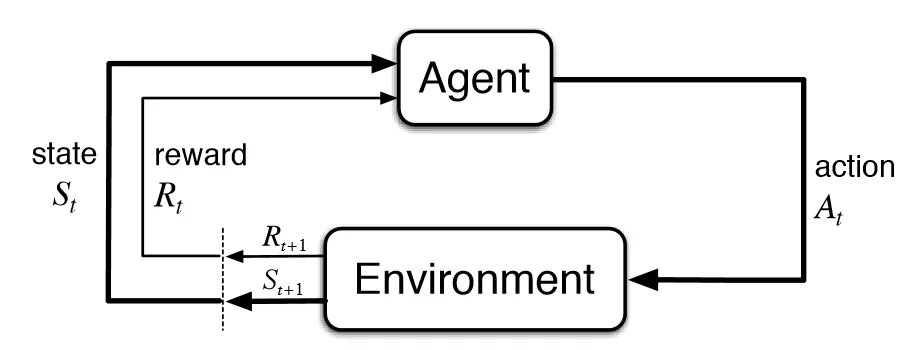
\includegraphics[width=0.6\textwidth]{Images/AgentEnvironment.png}
\caption{Interaction between the agent and the environment in a Reinforcement Learning setting.}
\label{Figure:AgentEnvironment}
\end{figure}

Figure \ref{Figure:AgentEnvironment} depicts the cyclical process of RL, highlighting the agent's decision-making loop: observation, action, and feedback. The agent continually adapts its policy to optimize behavior, ensuring alignment with the objectives encoded in the reward function, and in doing so, strives to maximize the expected return.

\subsubsection{Value Functions and Q-Functions}

In reinforcement learning, the value function and Q-function are vital tools for estimating the expected cumulative reward that an agent can achieve, which guide the agent's learning process. The Bellman equations, named after Richard Bellman, provide a recursive decomposition for the total cumulative reward an agent can expect to receive starting from a particular state or state-action pair. These equations are fundamental to dynamic programming techniques in RL, as they express the relationship between the value of the current state or action and the expected values of subsequent states or actions.

The value function for a policy \( \pi \), denoted as \( V^\pi(s) \), represents the expected return when starting in state \( s \) and following policy \( \pi \) thereafter. It is formulated as:

\begin{equation}
V^\pi(s) = \mathbb{E} \left[ \sum_{k=0}^{\infty} \gamma^k R_{t+k+1} \mid S_t = s, \pi \right]
\end{equation}

This is a non-recursive definition, relying on the expectation of the sum of discounted rewards when following policy \( \pi \). The corresponding Bellman equation for \( V^\pi(s) \) provides a recursive decomposition of this value function:

\begin{equation}
V^\pi(s) = \sum_{a \in A} \pi(a|s) \sum_{s' \in S} P(s'|s,a) \left[ R(s,a,s') + \gamma V^\pi(s') \right]
\end{equation}

The Q-function for a policy \( \pi \), \( Q^\pi(s, a) \), is the expected return for taking an action \( a \) in state \( s \) and following policy \( \pi \) afterwards:

\begin{equation}
Q^\pi(s, a) = \mathbb{E} \left[ \sum_{k=0}^{\infty} \gamma^k R_{t+k+1} \mid S_t = s, A_t = a, \pi \right]
\end{equation}

Similar to the value function, the Q-function also has its Bellman equation, which relates the Q-value of a state-action pair to the expected rewards plus the discounted future Q-values under policy \( \pi \):

\begin{equation}
Q^\pi(s, a) = \sum_{s' \in S} P(s'|s,a) \left[ R(s,a,s') + \gamma \sum_{a' \in A} \pi(a'|s') Q^\pi(s', a') \right]
\end{equation}

The relationship between the value function and the Q-function is given by:

\begin{equation}
V^\pi(s) = \sum_{a \in A} \pi(a|s) Q^\pi(s, a)
\end{equation}

This relationship indicates that the value of a state under policy \( \pi \) is the expected value of the Q-function over all possible actions, weighted by the policy's action probabilities.

For optimal policies, we define the optimal value function \( V^*(s) \) and the optimal Q-function \( Q^*(s, a) \), which represent the maximum possible returns achievable from any state or state-action pair, respectively:

\begin{equation}
V^*(s) = \max_{a \in A} \sum_{s' \in S} P(s'|s,a) \left[ R(s,a,s') + \gamma V^*(s') \right]
\end{equation}
\begin{equation}
V^*(s) = \max_{a \in A} Q^*(s, a)
\end{equation}
\begin{equation}
Q^*(s, a) = \sum_{s' \in S} P(s'|s,a) \left[ R(s,a,s') + \gamma \max_{a' \in A} Q^*(s', a') \right]
\end{equation}

The Bellman optimality equation for the Q-function expresses the idea that the optimal Q-value for a state-action pair is the immediate reward plus the discounted maximum future Q-values achievable from the next state.

Through iterative application of these equations, RL algorithms gradually approximate the value and Q-functions, guiding the agent towards the optimal policy that maximizes the expected cumulative reward.

\subsubsection{Methodological Variants and Learning Methods}

The methods of learning in reinforcement learning can be categorized along several axes: model-based versus model-free, on-policy versus off-policy, and value-based versus policy-based strategies.

Model-based RL algorithms create an explicit model of the environment, which they use to simulate the consequences of actions and make decisions. This approach is powerful when a precise model can be learned, as it allows the agent to plan by forecasting future states. Conversely, model-free RL algorithms do not attempt to model the environment; instead, they learn a policy or value function directly from experience gathered through interaction with the environment. Model-free approaches are often preferred in complex environments where modeling is impractical or when an accurate model is not available.

Within the model-free paradigm, there are on-policy methods, which learn about the policy that is currently used to make decisions, and off-policy methods, which learn about a different, potentially optimal policy while following a different policy for exploring the environment.

Additionally, a fundamental distinction is made between value-based and policy-based learning. Value-based methods, such as Temporal Difference (TD) Learning, Q-learning, and SARSA, focus on estimating the value of states or state-action pairs, with policies derived implicitly from these values. All three algorithms are examples of model-free and on-policy (SARSA) or off-policy (Q-learning and TD Learning) methods.

Policy-based methods, such as the REINFORCE algorithm, directly optimize the policy. These methods are particularly beneficial in scenarios where the action space is either high-dimensional or continuous. Actor-Critic methods, however, embody a hybrid approach, featuring both a policy function (the actor) and a value function (the critic), hence offering the stability and efficiency of value-based methods with the direct policy improvement of policy-based methods.

The Actor-Critic algorithm is especially pertinent to our research. Serving as a bridge to the more advanced deep deterministic policy gradient (DDPG) algorithm—a sophisticated actor-critic method that utilizes deep learning—the foundational Actor-Critic approach is instrumental. It employs a dual system where the actor updates the policy based on the sampled data, and the critic assesses the action as per the current policy. This synergy provides refined policy updates, which is particularly advantageous in the intricate and unpredictable domain of forex trading. The pseudo-code for the Actor-Critic algorithm, as seen in Algorithm~\ref{Code:ActorCritic}, delineates this process.

\begin{algorithm}[htb!]
\caption{Actor-Critic}
\label{Codes:ActorCritic}
\begin{algorithmic}
\REQUIRE $\pi(s, a; \theta)$: a differentiable policy, $Q(s, a; w)$: a differentiable $Q$-function, $N$: number of iterations and learning rates $\beta^\theta > 0$ and $\beta^w > 0$
\STATE Initialize policy parameter $\theta^{(0)}$ and $Q$-function parameter $w^{(0)}$
\STATE Initialize state $s$
\FOR{$n = 0, 1, \ldots, N - 1$}
    \STATE Sample $a \sim \pi(s, a; \theta^{(n)})$
    \STATE Take action $a$, observe state $s'$ and reward $r$
    \STATE Sample action $a' \sim \pi(s', a; \theta^{(n)})$
    \STATE Compute the TD error: $\delta \gets r + \gamma Q(s', a'; w^{(n)}) - Q(s, a; w^{(n)})$
    \STATE Update $w$: $w^{(n+1)} \gets w^{(n)} + \beta^w \delta \nabla_w Q(s, a; w^{(n)})$
    \STATE Update $\theta$: $\theta^{(n+1)} \gets \theta^{(n)} + \beta^\theta \delta \nabla_\theta \ln \pi(s, a; \theta^{(n)})$
    \STATE $s \gets s'$, $a \gets a'$
\ENDFOR
\end{algorithmic}
\end{algorithm}


It is crucial to recognize that while the Puterman theorem offers convergence assurances for MDPs, affirming the existence of a deterministic stationary optimal policy, such guarantees are not directly transferable to the multifaceted arenas like financial markets. The forex market, for instance, does not conform to a state representation that fully captures historical information, due to the inherent influence of past data on current states. Therefore, applying RL to such domains involves working with approximations of these theoretical models. Through the application of technical indicators and meticulous feature engineering, we strive to encapsulate as much pertinent historical information as possible within the state representation. The DDPG algorithm, which builds upon the Actor-Critic framework with the power of neural networks, is aptly suited for this complex task and will be the centerpiece of the forthcoming section on Deep Reinforcement Learning.

\subsection{Deep Reinforcement Learning}

Deep Reinforcement Learning (DRL) combines the decision-making prowess of reinforcement learning with the pattern recognition capabilities of neural networks. This fusion is particularly potent in domains characterized by complex, high-dimensional data, such as the forex market. DRL equips trading algorithms with the adaptability required to thrive in such volatile environments, potentially revolutionizing trading strategies with its capacity for continuous learning and adaptation.

\subsubsection{Fundamentals and History}
The emergence of DRL as a distinct field within artificial intelligence was propelled by the realization that neural networks could significantly amplify the ability of reinforcement learning agents to interact with and learn from complex environments. The early days of neural network research laid the groundwork for such integrative approaches, with the development of algorithms capable of learning rich representations from raw data.

DeepMind's landmark work, showcasing the Deep Q-Network (DQN) algorithm's success in mastering a suite of Atari 2600 games from visual inputs alone, signified a major breakthrough for DRL. This achievement not only validated the efficacy of DRL in mastering high-dimensional state spaces but also highlighted its potential applicability to financial markets. Here, the challenge is not only to interpret vast arrays of data but also to derive from them a strategic understanding that can guide trading decisions in real time.

This historical advance, along with ongoing research, has galvanized interest in applying DRL to forex trading. The field's evolution reflects a broader ambition: to harness the intricacy of market signals and evolve strategies that are resilient and dynamic. It is this ambition that informs the current drive to adapt DRL methodologies to the domain of forex trading, where the ability to learn from and capitalize on complex market dynamics is paramount.

\subsubsection{Deep Value-Based RL Algorithms: Deep Q-Networks}

The advent of deep learning has transformed traditional value-based reinforcement learning methods, giving rise to what is known today as Deep Value-Based Methods. These advanced algorithms employ neural networks, renowned for their function approximation capabilities, to manage and interpret larger state spaces. Such an approach enables agents to learn and operate effectively in environments with complex, high-dimensional sensory input, a task that conventional value-based methods could not scale to efficiently.

Neural Fitted Q-Learning was one of the early techniques that laid the foundation for deep value-based learning. It utilizes neural networks to approximate the Q-function, which represents the expected return of a given state-action pair. By fitting a neural network to the Q-values obtained from completed episodes, it significantly enhanced the agent's ability to generalize across states in large and continuous spaces.

The field of Deep Value-Based Methods truly came into prominence with the introduction of the Deep Q-Network (DQN) algorithm by Mnih et al. DQN integrated key innovations such as a separate target network for stabilizing the learning targets and an experience replay mechanism for breaking the temporal correlations within training batches. This approach allowed DQN to effectively learn control policies directly from high-dimensional inputs, a significant leap forward in the application of RL.

Following DQN, improvements such as the Double Deep Q-Network (DDQN) sought to address issues inherent in the DQN architecture. DDQN mitigates the overestimation bias of action values by decoupling the action selection from the action evaluation. This is achieved by employing two networks: a primary network for action selection and a target network for evaluation, enhancing the stability and accuracy of the value estimation process.

The deep value-based methods, while foundational and revolutionary, will not be the primary focus of the current research proposal. The research will instead concentrate on Deep Policy-Based Methods, as we will see in the next section.

\subsubsection{Deep Policy-Based RL Algorithms: Deep Deterministic Policy Gradient}

Deep Policy-Based Reinforcement Learning Algorithms excel in environments with continuous action spaces. Unlike value-based methods that assign a value to each potential action, policy-based approaches directly optimize the policy to maximize expected returns. This quality is invaluable in the domain of forex trading, characterized by a vast and continuous action space that demands both precision and adaptability.

Within this category, the Deep Deterministic Policy Gradient (DDPG) algorithm emerges as a prominent model-free, off-policy actor-critic method designed for continuous action spaces. By blending the direct policy optimization of policy-based methods with the evaluative power of value-based approaches, DDPG achieves a stable and robust learning process. The algorithm is structured around an actor, responsible for action selection, and a critic that appraises the actions by estimating their Q-values.

\begin{algorithm}[htb!]
\caption{Deep Deterministic Policy Gradient}
\label{Code:DeepDeterministicPolicyGradient}
\begin{algorithmic}
\REQUIRE an actor $\pi(s; \theta)$, a critic network $Q(s, a; \phi)$, learning rates $\beta$ and $\hat{\beta}$, initial parameters $\theta^{(0)}$ and $\phi^{(0)}$
\STATE Initialize target network parameters $\hat{\phi} \leftarrow \phi^{(0)}$ and $\hat{\theta} \leftarrow \theta^{(0)}$, replay buffer $\mathcal{B}$
\FOR{episode $= 1, M$}
    \STATE Initialize a random process $\mathcal{N}$ for action exploration
    \STATE Receive initial observation state $s_1$
    \FOR{t $= 1, T$}
        \STATE Select action $a_t = \pi(s_t; \theta) + \mathcal{N}_t$ according to the current policy and exploration noise
        \STATE Execute action $a_t$ and observe reward $r_t$ and new state $s_{t+1}$
        \STATE Store transition $(s_t, a_t, r_t, s_{t+1})$ in $\mathcal{B}$
        \STATE Sample a random minibatch of $N$ transitions $(s_i, a_i, r_i, s_{i+1})$ from $\mathcal{B}$
        \STATE Set $y_i = r_i + \gamma Q'(s_{i+1}, \pi'(s_{i+1}; \hat{\theta}); \hat{\phi})$
        \STATE Update critic by minimizing the loss: $L = \frac{1}{N}\sum_i(y_i - Q(s_i, a_i; \phi))^2$
        \STATE Update the actor policy using the sampled policy gradient:
        \STATE $\nabla_{\theta} J \approx \frac{1}{N}\sum_i \nabla_a Q(s, a; \phi)|_{s=s_i, a=\pi(s_i)} \nabla_{\theta}\pi(s; \theta)|_{s_i}$
        \STATE Update the target networks:
        \STATE $\hat{\phi} \leftarrow \tau \phi + (1 - \tau) \hat{\phi}$
        \STATE $\hat{\theta} \leftarrow \tau \theta + (1 - \tau) \hat{\theta}$
    \ENDFOR
\ENDFOR
\end{algorithmic}
\end{algorithm}


Algorithm~\ref{Code:DeepDeterministicPolicyGradient} demonstrates DDPG's employment of deep neural networks to approximate the actor and the critic functions, enabling the processing of complex input dimensions typical of forex markets. The utilization of a replay buffer for experience storage and the strategic sampling of mini-batches are key features that enhance learning stability by mitigating the correlation between sequential data points. Furthermore, DDPG incorporates target networks, which are gradually updated versions of the actor and critic, to solidify the learning targets and foster gradual improvement.

While the convergence of DDPG is not categorically assured—owing to the dynamic and partially observable nature of forex markets—the algorithm's design for continual policy adaptation offers a compelling approach for developing sophisticated trading strategies. The adaptability of DDPG to the evolving conditions of financial markets underscores its potential as a significant advancement in the realm of algorithmic trading. The next section, will delve into existing literature and studies, shedding light on how other researchers have approached the challenges of forex trading with reinforcement learning and where DDPG situates within this broader context.
